\begin{appendices}
\label{appendix:graph}
	\chapter{Реализованный web-интерфейс}
	
	На рисунках \ref{img:home}~--~\ref{img:ad} представлен web-интерфейса.
	
\begin{figure}[h!]
	\centering
    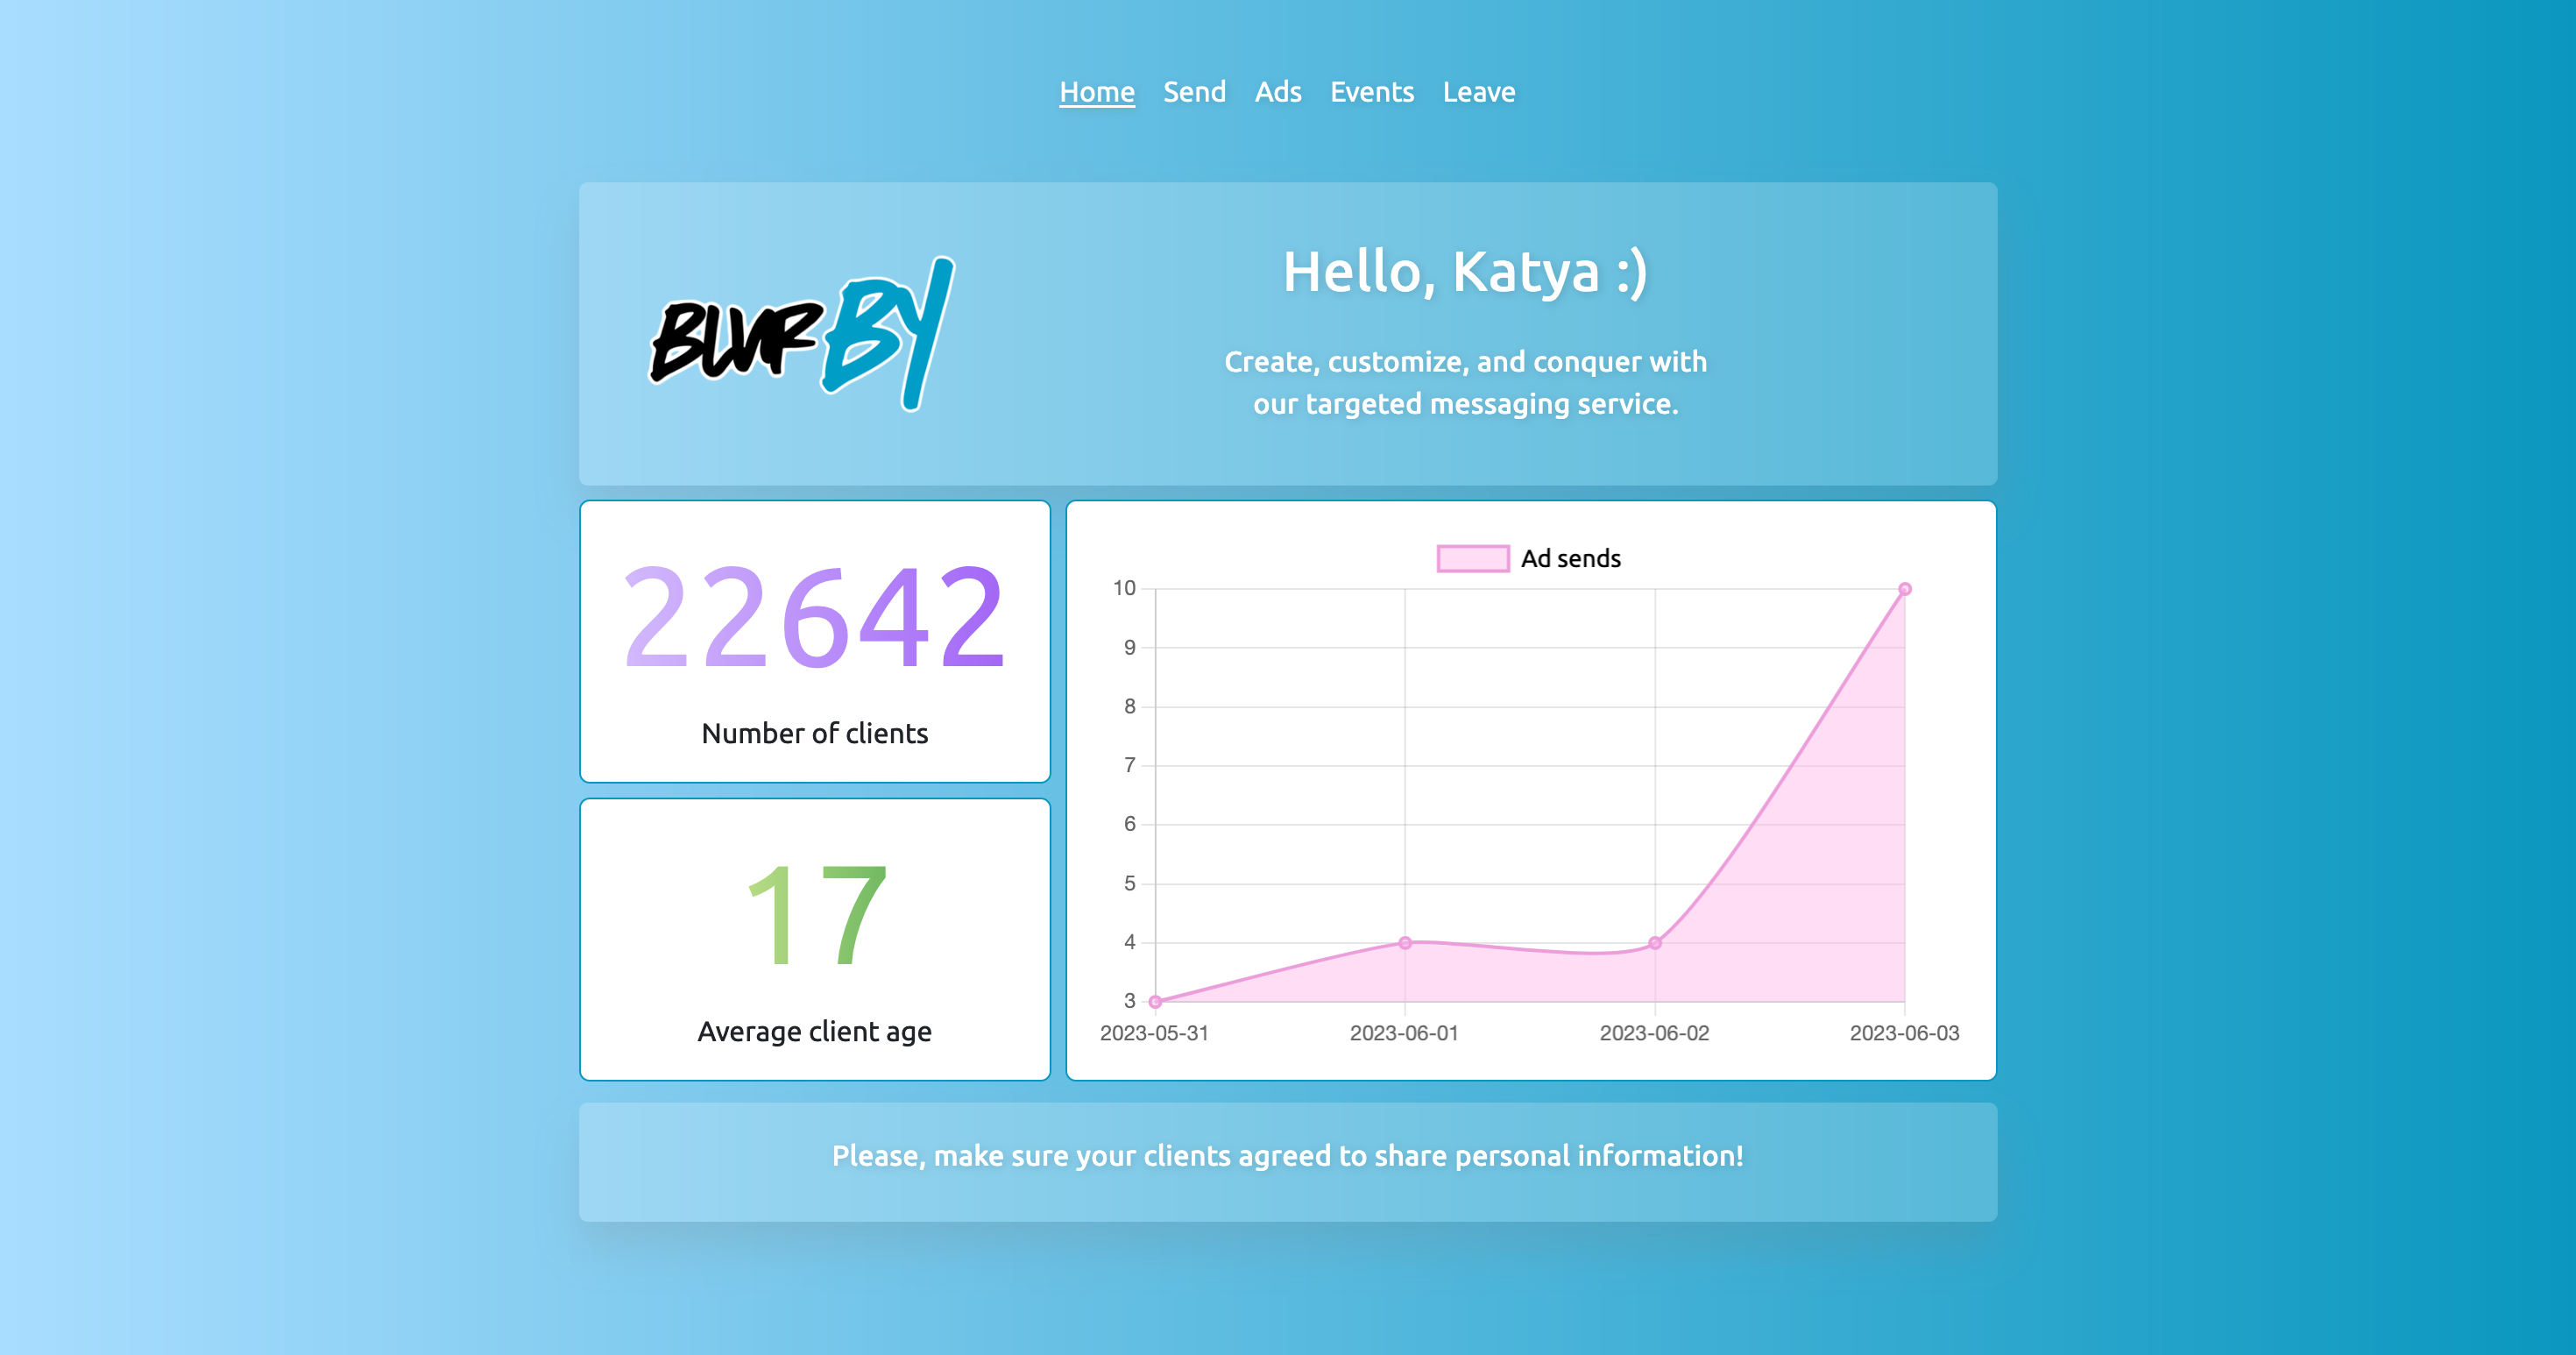
\includegraphics[width=\linewidth]{./images/home.png}
    \caption{Домашняя страница}
    \label{img:home}
\end{figure}

\begin{figure}[h!]
	\centering
    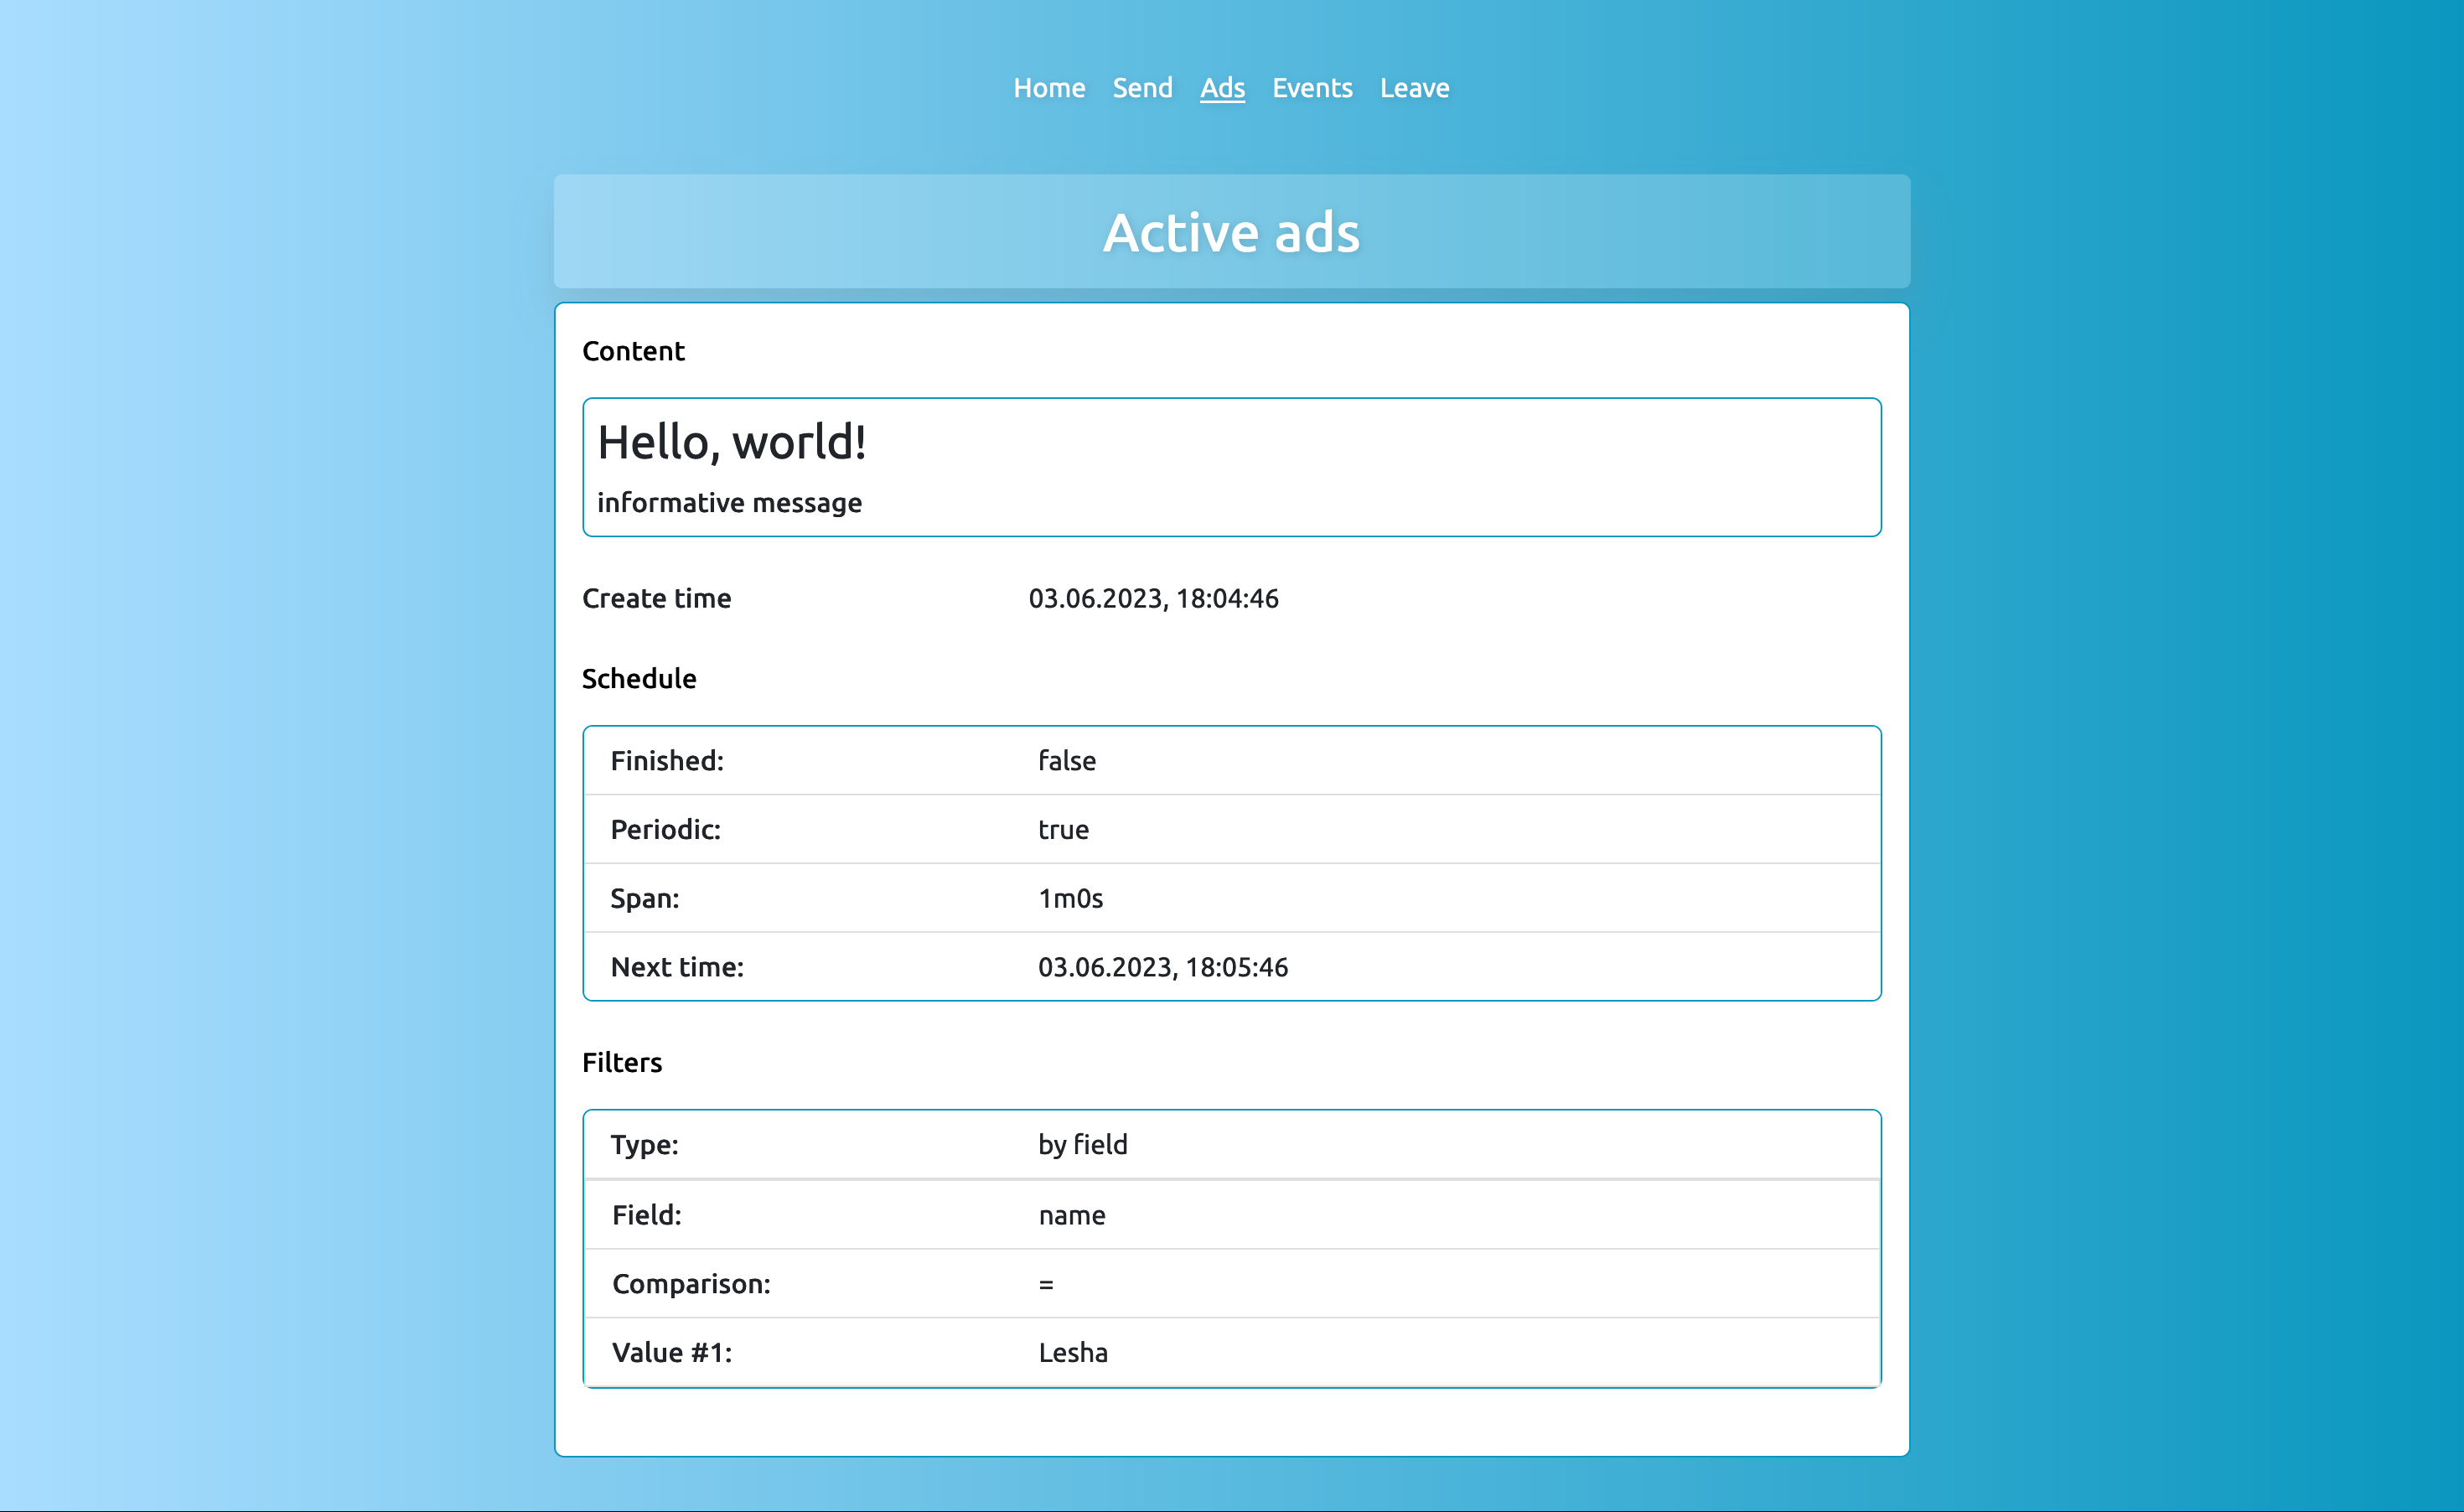
\includegraphics[width=\linewidth]{./images/ads.png}
    \caption{Страница просмотра списка незавершённых рассылок}
    \label{img:ads}
\end{figure}

\newpage

\begin{figure}[h!]
	\centering
    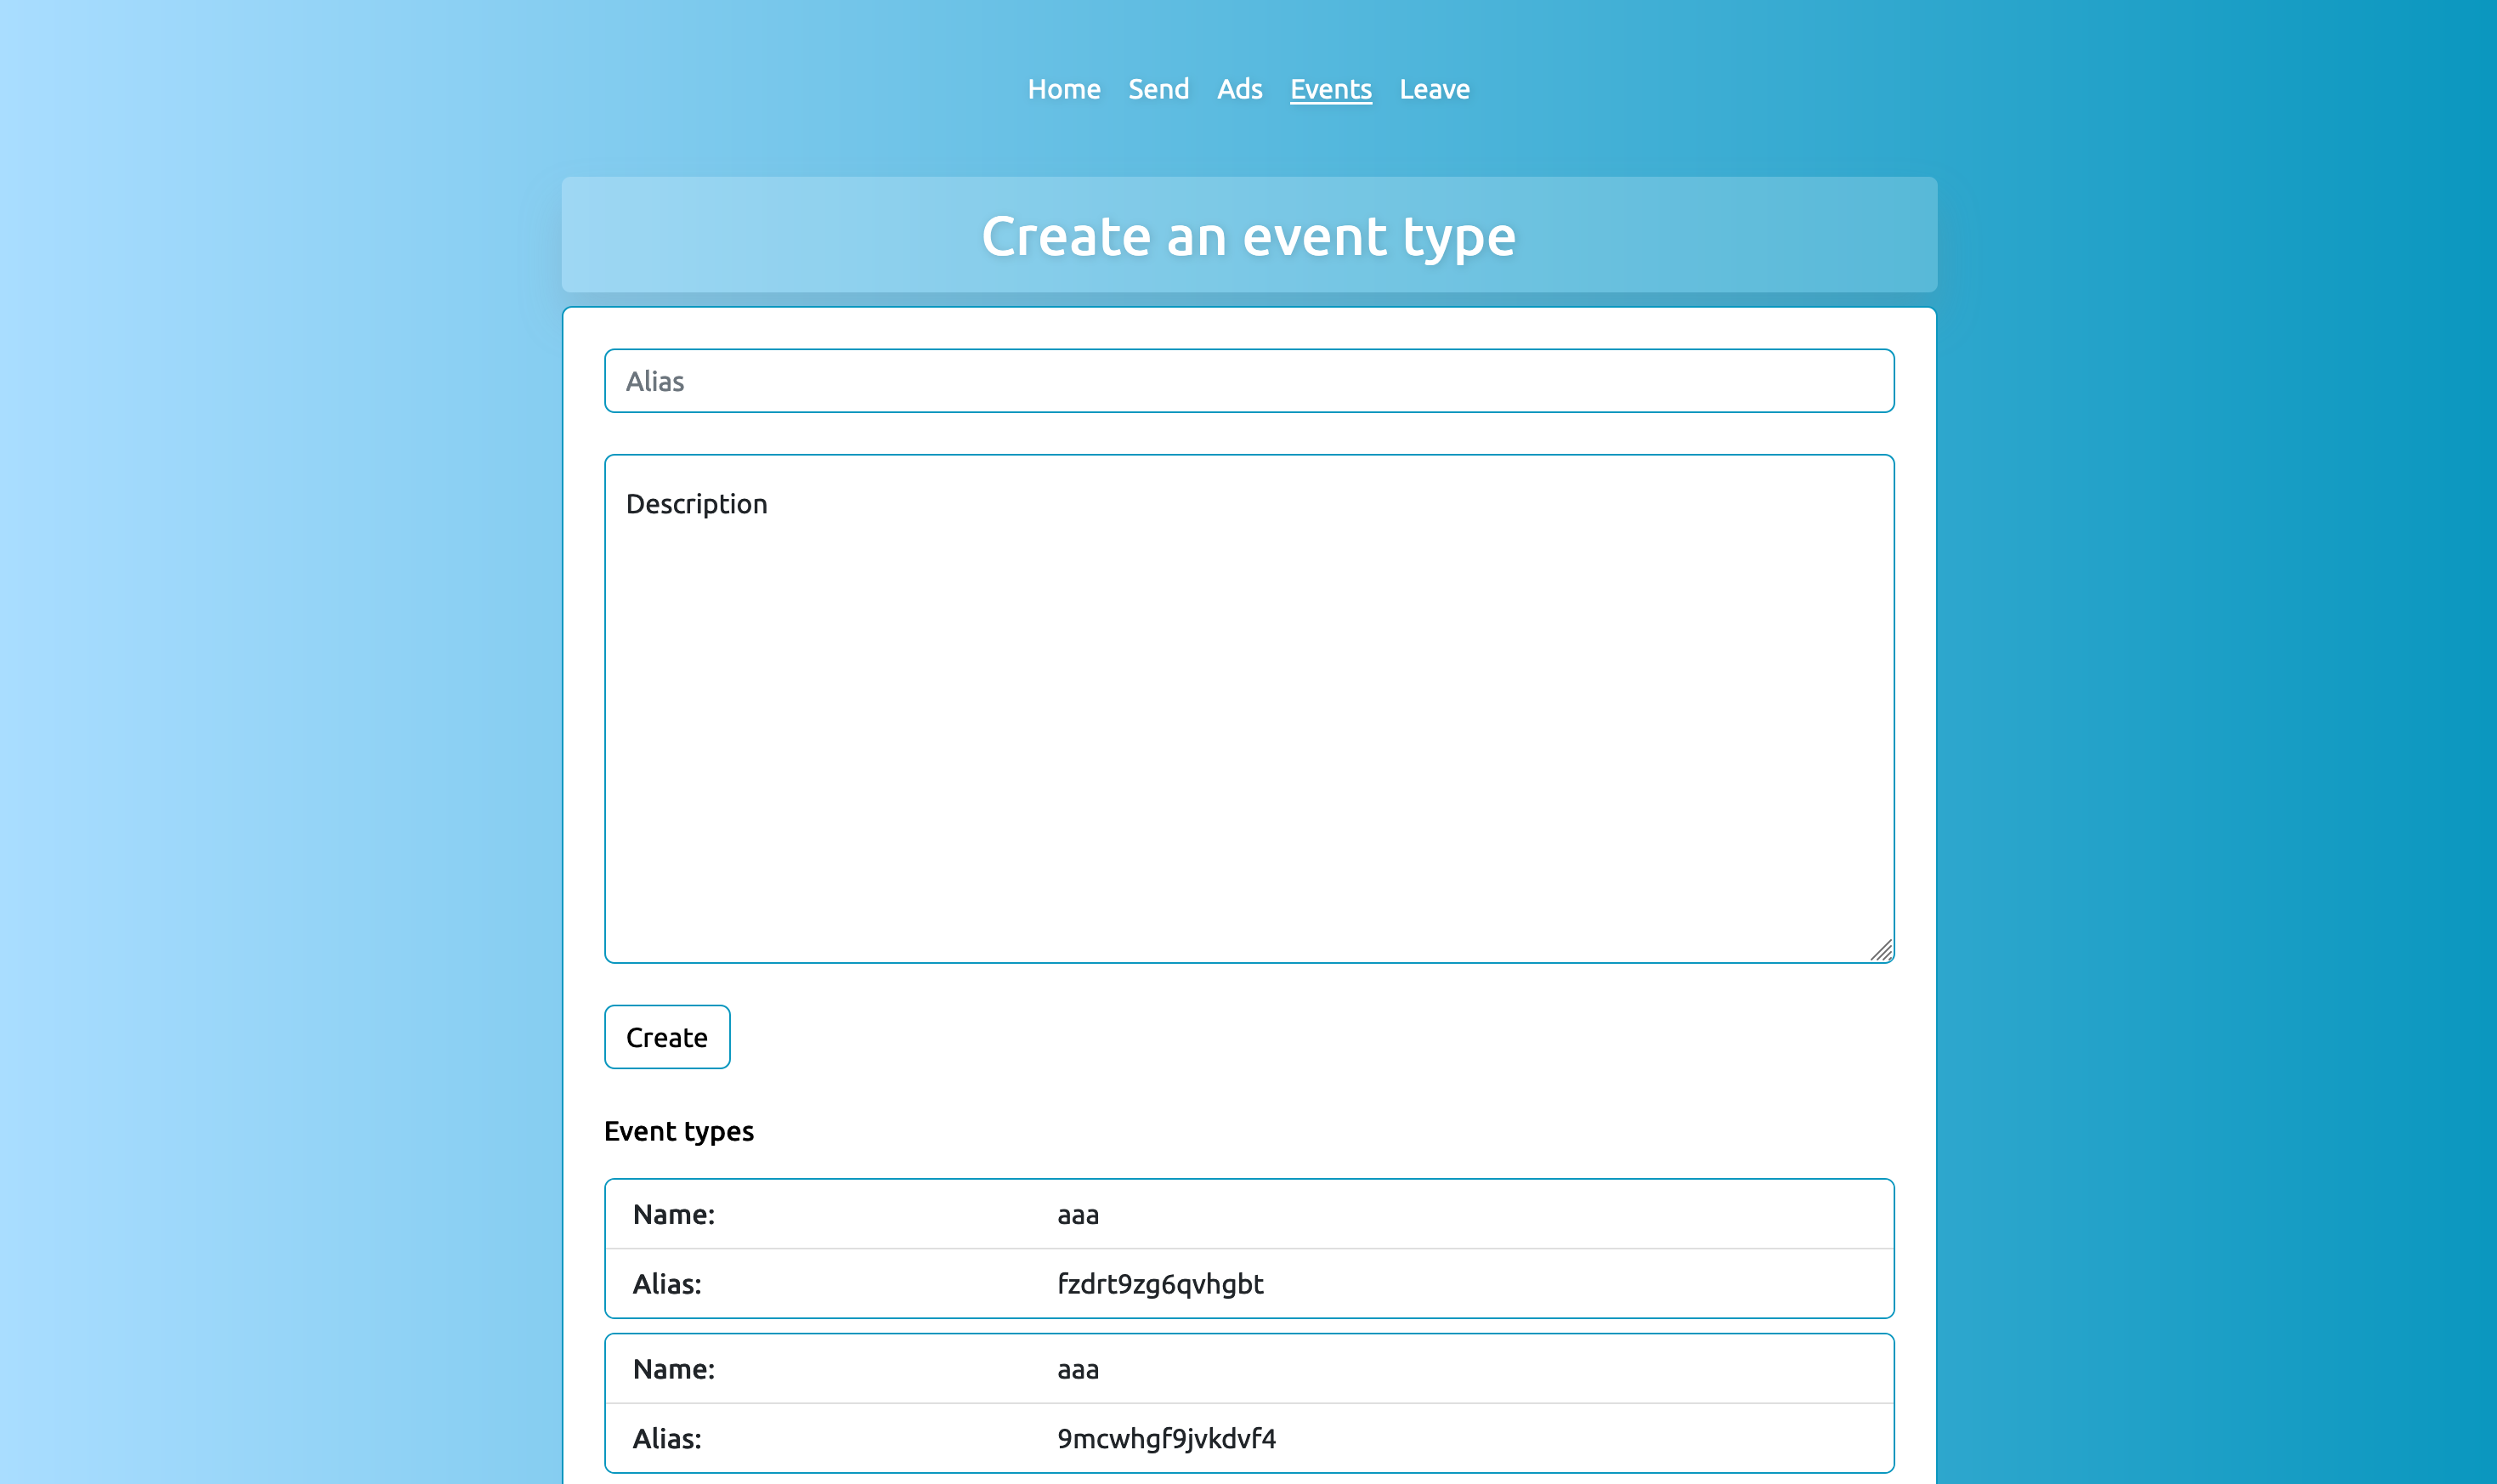
\includegraphics[width=\linewidth]{./images/ets.png}
    \caption{Страница просмотра и создания типов событий}
    \label{img:ets}
\end{figure}

\begin{figure}[h!]
	\centering
    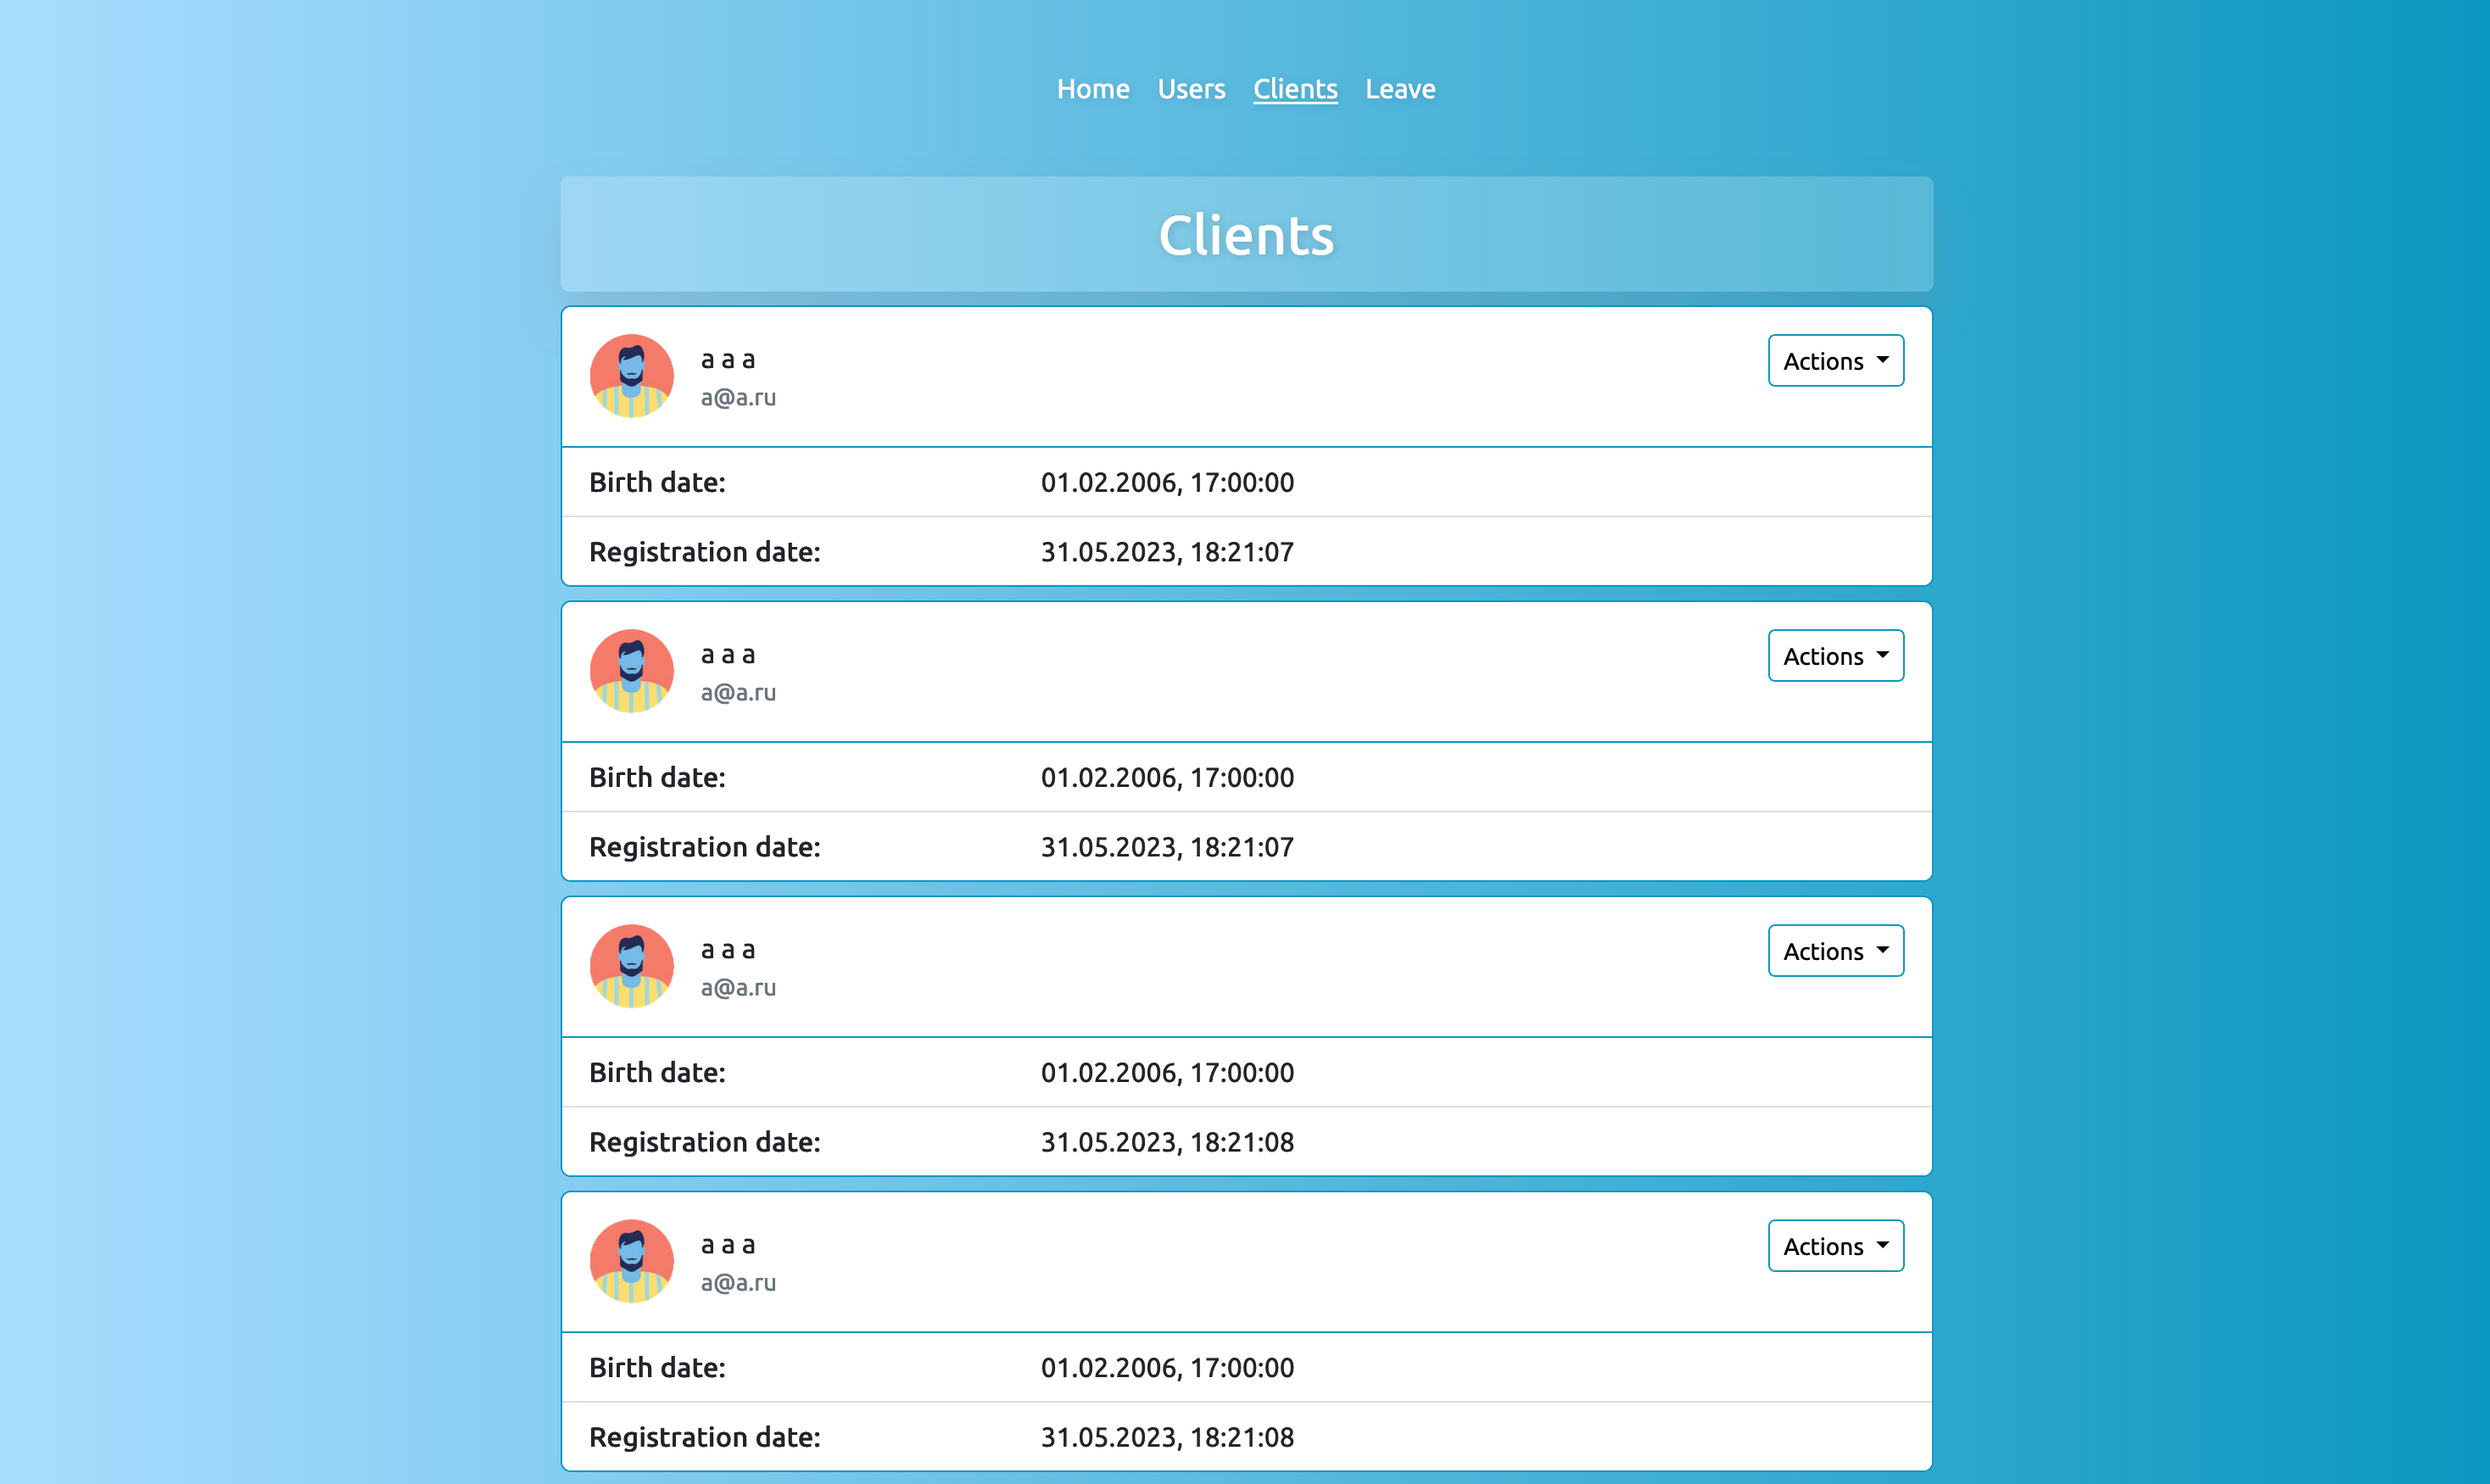
\includegraphics[width=\linewidth]{./images/clients.png}
    \caption{Страница просмотра и редактирования списка клиентов}
    \label{img:clients}
\end{figure}

\newpage

\begin{figure}[h!]
	\centering
    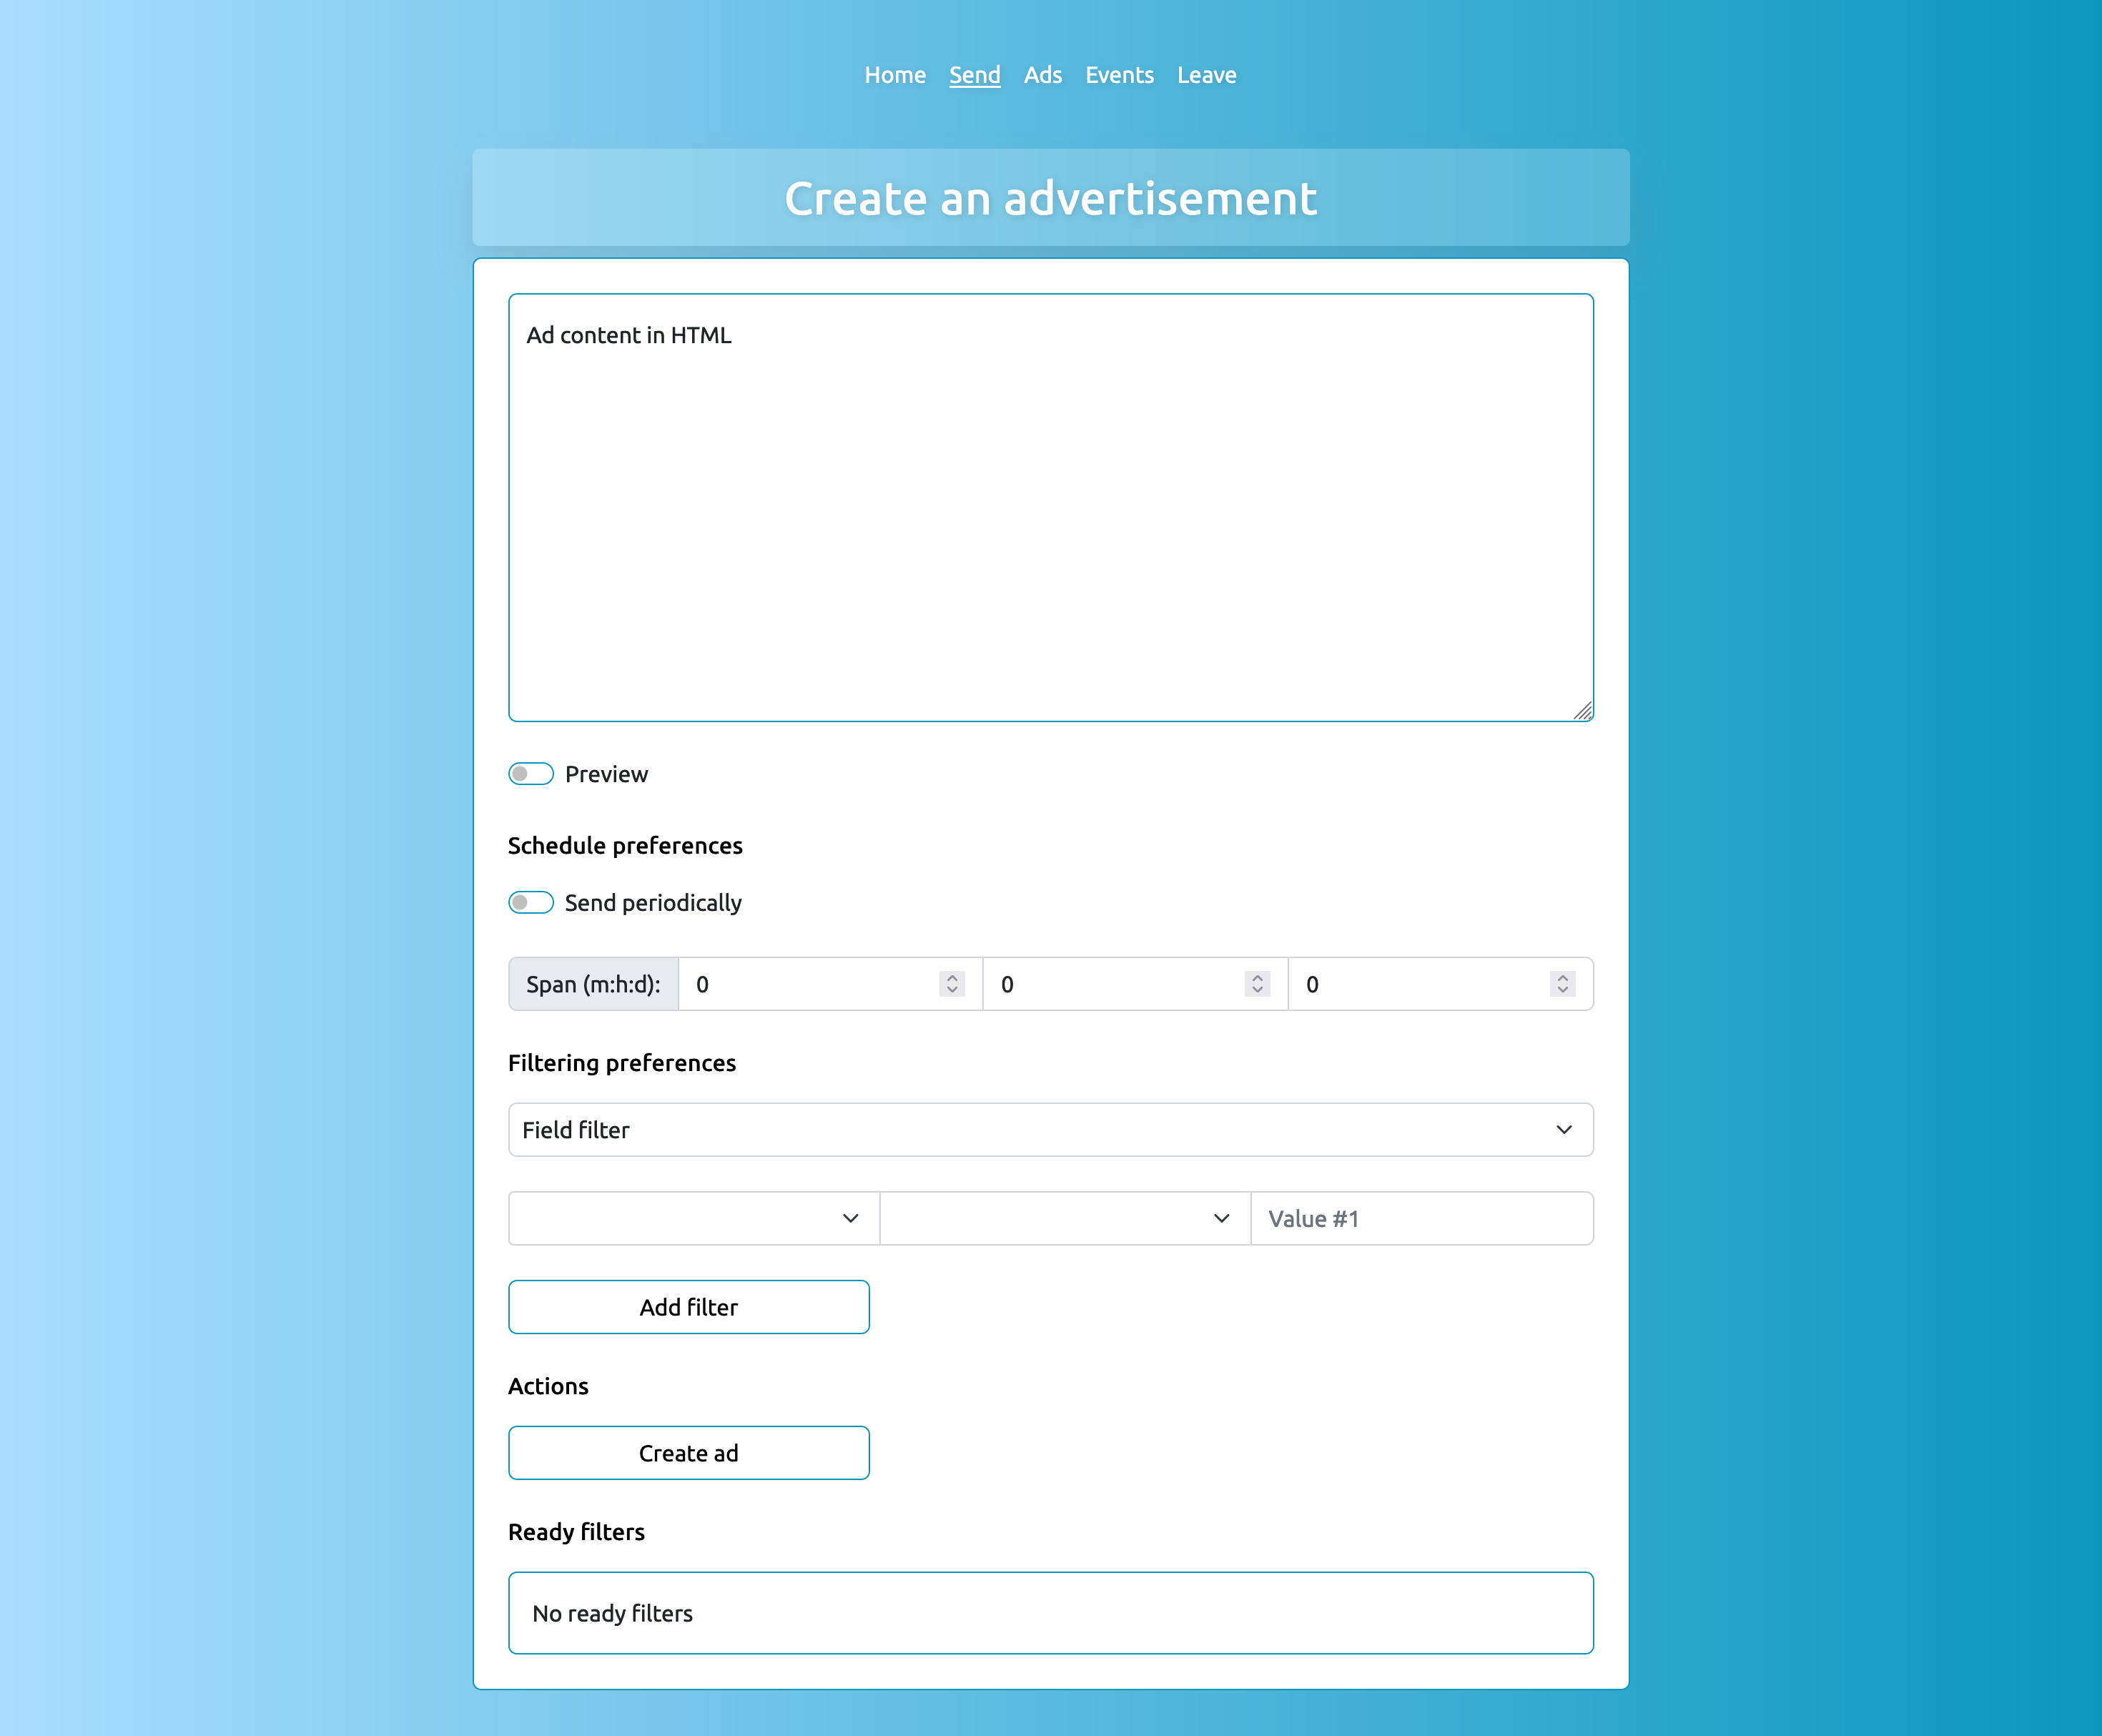
\includegraphics[width=\linewidth]{./images/ad.png}
    \caption{Страница формирования рекламной рассылки}
    \label{img:ad}
\end{figure}


\newpage

	
\end{appendices}